%% XeLaTeX — compile with: xelatex main.tex
\documentclass[10pt,twocolumn]{article}

\usepackage{geometry}
\geometry{a4paper, top=2.0cm, bottom=2.0cm, left=1.6cm, right=1.6cm, columnsep=0.6cm}

\usepackage{fontspec}
\setmainfont{Times New Roman}
\setsansfont{Helvetica Neue}
\setmonofont[Scale=0.85]{Menlo}

\usepackage{microtype}
\usepackage{graphicx}
\usepackage{booktabs}
\usepackage{amsmath,amssymb}
\usepackage{xcolor}
\usepackage{hyperref}
\usepackage{caption}
\usepackage{subcaption}
\usepackage{enumitem}
\usepackage{titlesec}
\usepackage{abstract}
\usepackage{parskip}
\usepackage{fancyhdr}
\usepackage{multirow}

\definecolor{dreamerblue}{HTML}{2166ac}
\definecolor{sacred}{HTML}{d6604d}
\definecolor{darkgray}{HTML}{333333}
\definecolor{lightgray}{HTML}{f5f5f5}

\hypersetup{
  colorlinks=true,
  linkcolor=dreamerblue,
  citecolor=dreamerblue,
  urlcolor=dreamerblue
}

\titleformat{\section}{\large\bfseries\sffamily}{}{0em}{}[\titlerule]
\titleformat{\subsection}{\normalsize\bfseries\sffamily}{}{0em}{}
\titlespacing*{\section}{0pt}{1.2ex plus .5ex}{0.8ex}
\titlespacing*{\subsection}{0pt}{0.9ex plus .3ex}{0.4ex}

\captionsetup{font=small, labelfont=bf, skip=4pt}

\pagestyle{fancy}
\fancyhf{}
\renewcommand{\headrulewidth}{0.4pt}
\fancyhead[L]{\small\sffamily\textcolor{darkgray}{Dreamer vs.\ SAC+VAE for Autonomous RC Car}}
\fancyhead[R]{\small\sffamily\textcolor{darkgray}{\thepage}}

% ─────────────────────────────────────────────────────────────────────────────
\begin{document}

\twocolumn[{%
\begin{@twocolumnfalse}

\vspace*{0.3cm}
{\noindent\Large\bfseries\sffamily
  Model-Based Reinforcement Learning for Autonomous RC Car Navigation:\\
  Dreamer versus SAC+VAE on the DonkeyCar Platform
}

\vspace{0.5em}
{\noindent\normalsize
  Harsh Wadhawe$^1$ \quad \texttt{harsh.wadhawe@tamu.edu}
  \qquad
  Guni Sharon$^1$ \quad \texttt{guni@tamu.edu}
  \\[0.3em]
  \small $^1$Texas A\&M University
}

\vspace{0.8em}
\hrule
\vspace{0.5em}

\begin{abstract}
\noindent
We compare two reinforcement learning approaches for training an autonomous
miniature car entirely from raw pixels: \textbf{Dreamer}, a model-based method
that learns a latent world model and optimises a policy via imagined rollouts, and
\textbf{SAC+VAE}, a model-free baseline that encodes observations with a
pre-trained $\beta$-VAE and trains a Soft Actor-Critic agent.
Both methods share an identical reward signal—survival bonus plus throttle,
with no cross-track error—ensuring results transfer to the physical hardware.
On the DonkeyCar generated track, Dreamer achieves its first complete lap in
\textbf{16 episodes} compared to \textbf{108 episodes} for SAC+VAE
(7$\times$ improvement in sample efficiency), with comparable wall-clock time
once VAE pre-training is included.
Dreamer's policy gradients remain stable; SAC+VAE exhibits Q-value divergence
when operating on a frozen encoder, a known limitation with model-free methods.
The trained Dreamer policy is exported as a TFLite graph and deployed on a
Raspberry Pi~5 at inference, demonstrating practical sim-to-real transfer.
\end{abstract}

\vspace{0.5em}
\hrule
\vspace{1.0em}

\end{@twocolumnfalse}
}]

% ─────────────────────────────────────────────────────────────────────────────
\section{Introduction}

Learning end-to-end visuomotor policies directly from raw camera images
is attractive for small autonomous platforms where adding dense sensing
(GPS, lidar) is impractical.
The DonkeyCar~\cite{donkeycar} ecosystem provides a simulator and a low-cost
RC car fitted with a single forward-facing camera, making it a concrete
testbed for this challenge.

Reinforcement learning from pixels has progressed substantially with
model-based approaches such as Dreamer~\cite{hafner2019dream,hafner2020dreamerv2,hafner2023dreamerv3},
which learn a compact latent world model and train an actor-critic
entirely through imagined experience.
In contrast, model-free algorithms such as
Soft Actor-Critic (SAC)~\cite{haarnoja2018sac} require orders of magnitude more
environment interaction but avoid the complexity of world-model training.

A common approach to reduce the sample cost of model-free methods on
image-based tasks is to decouple representation learning: train a
variational autoencoder (VAE)~\cite{kingma2014vae} offline on collected frames,
then freeze the encoder and train SAC on latent codes~\cite{ha2018worldmodels}.
This SAC+VAE pipeline serves as our model-free baseline.

Our contributions are:
\begin{itemize}[leftmargin=1.2em, itemsep=1pt, topsep=2pt]
  \item A principled reward formulation (survival + throttle, no cross-track error)
        that transfers directly to the physical car without simulator-specific signals.
  \item A systematic wall-clock comparison that includes all setup costs:
        data collection and VAE pre-training for SAC+VAE,
        and seed-episode collection for Dreamer.
  \item A reduced-size Dreamer architecture (\S\ref{sec:dreamer}) tuned for
        fast TFLite inference on the Raspberry Pi~5.
  \item Empirical demonstration of 7$\times$ sample efficiency of Dreamer
        over SAC+VAE on the DonkeyCar generated track.
\end{itemize}

% ─────────────────────────────────────────────────────────────────────────────
\section{Background}

\subsection{Dreamer}
Dreamer~\cite{hafner2019dream} learns a Recurrent State Space Model (RSSM)
consisting of a deterministic GRU belief $h_t$ and a Gaussian stochastic state
$z_t$. At each step the world model predicts the next state, reconstructs the
observation, and estimates the scalar reward. An actor-critic policy is then
optimised purely through differentiable rollouts of length $H$ inside the latent
space, requiring no additional environment steps during policy updates.

DreamerV2~\cite{hafner2020dreamerv2} introduced KL balancing and
categorical latents. DreamerV3~\cite{hafner2023dreamerv3} added symlog
reward transforms and return normalisation. Our implementation is a hybrid:
Gaussian stochastic states with KL balancing (V2), symlog rewards, and return
normalisation (V3), without the twohot distributional critic.

\subsection{SAC+VAE}
Soft Actor-Critic~\cite{haarnoja2018sac} maximises a maximum-entropy objective
$J(\pi) = \mathbb{E}[\sum_t r_t + \alpha \mathcal{H}(\pi(\cdot|s_t))]$
using twin Q-networks and auto-tuned temperature $\alpha$.
When the observation is a raw image, a common approach is to pre-train
a $\beta$-VAE~\cite{higgins2017betavae} on collected frames, freeze the encoder,
and feed the latent mean $z = \mu_\phi(o)$ to the SAC agent.
This avoids end-to-end gradient flow through a convolutional encoder during
Q-learning, at the cost of a fixed, non-adaptive representation.

% ─────────────────────────────────────────────────────────────────────────────
\section{Method}

\subsection{Observation Pipeline}
Both methods share the same preprocessing: the top 40 rows of the
$120\times160$ camera image are cropped (sky / roof), the result is
resized to $64\times64$ pixels, and normalised to $[-0.5, 0.5]$.
RGB (3-channel) images are used throughout.

\subsection{Reward Design}
\label{sec:reward}

A core design constraint is that every signal in the reward must be
observable on the physical car at inference time.
Cross-track error (CTE) is available in the DonkeyCar simulator
via Unity physics, but is unavailable on hardware.
We therefore define:
\[
  r_t = \underbrace{r_\text{surv}}_{\text{0.5}} +\; \underbrace{a_t^\text{throttle}}_{\in[0,0.4]}
\]
where $r_\text{surv}=0.5$ is a constant survival bonus added at each step
the car remains on track.
The throttle contribution rewards forward progress and encourages the agent
to learn speed management rather than simply surviving at crawl speed.
A full 1000-step episode yields a maximum reward of approximately $840$.

CTE is used exclusively for episode termination in automated training mode:
the episode ends if $\text{cte} > 2.0$ (off-road right)
or $\text{cte} < -6.0$ (off-road left), with asymmetric bounds to account
for the track reference being the right lane.

\subsection{Dreamer Architecture}
\label{sec:dreamer}

We use a reduced RSSM to lower TFLite inference latency on the Pi~5
and reduce risk of over-fitting simulator-specific textures:

\begin{table}[h]
\centering\small
\caption{RSSM architecture (ours vs.\ DreamerV2).}
\label{tab:arch}
\begin{tabular}{lrr}
\toprule
Parameter & Ours & DreamerV2 \\
\midrule
Belief size    & 128  & 200  \\
State size     & 20   & 30   \\
Hidden size    & 200  & 400  \\
Embedding size & 512  & 1024 \\
\bottomrule
\end{tabular}
\end{table}

The CNN encoder uses four convolutional layers with ReLU activations and
outputs a 512-dimensional embedding. The policy is a four-layer MLP
producing a TanhNormal distribution over steering and throttle.
Twin critics share the same architecture but maintain separate parameters.
The full policy graph (encoder + RSSM + actor) is exported via
\texttt{torch.export} and compiled to TFLite for on-device inference.

\begin{figure*}[t]
  \centering
  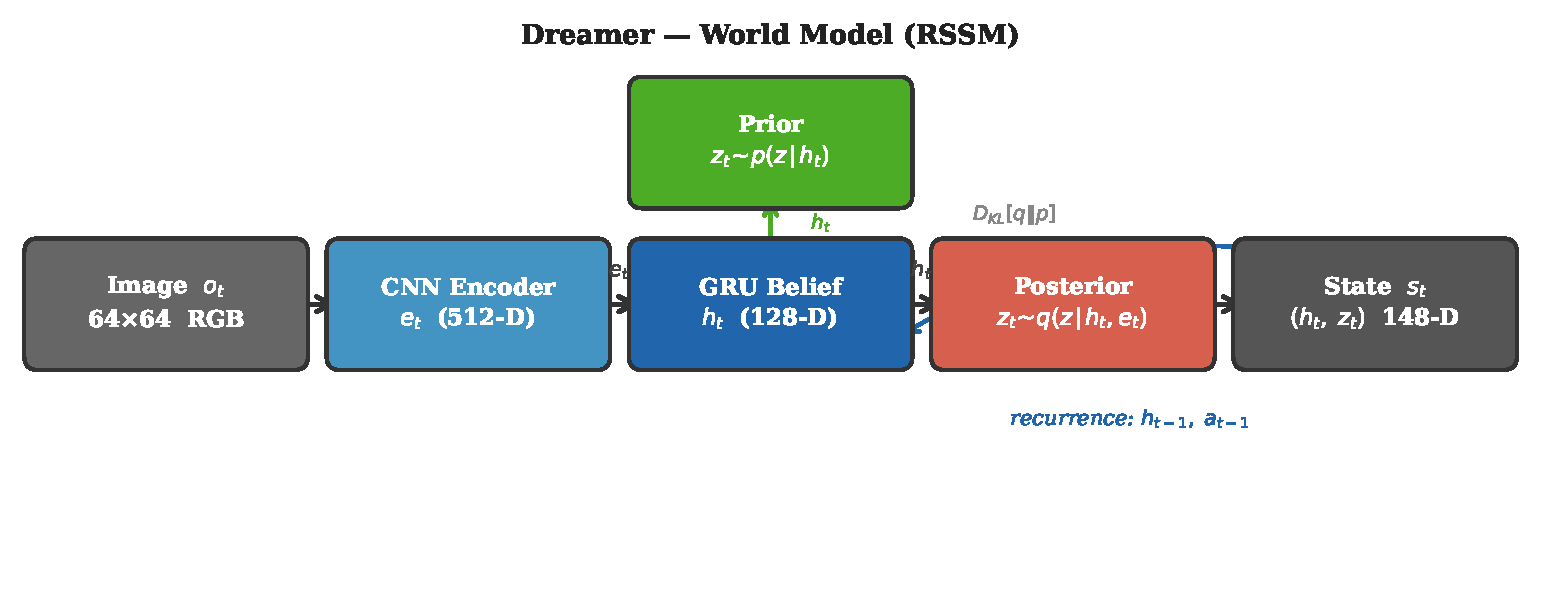
\includegraphics[width=0.95\textwidth]{figures/dreamer_rssm.pdf}\\[0.6em]
  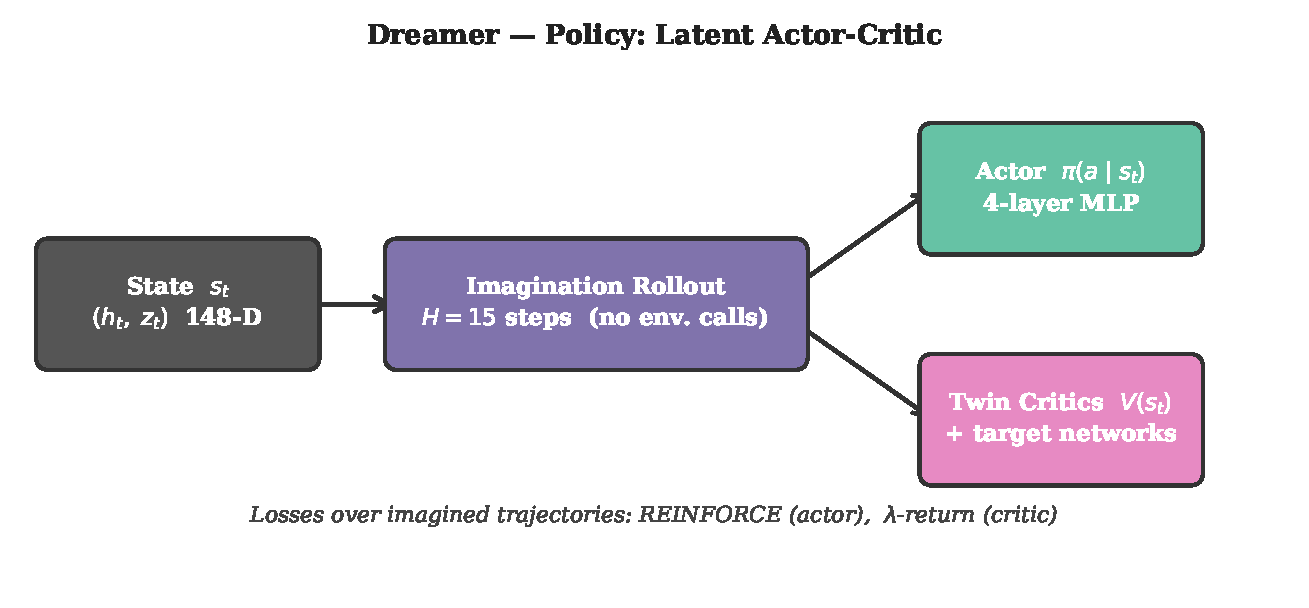
\includegraphics[width=0.70\textwidth]{figures/dreamer_policy.pdf}
  \caption{Dreamer architecture.
    \emph{Top — World Model (RSSM):} A CNN encoder produces embedding $e_t$.
    The GRU updates deterministic belief $h_t$; a Gaussian posterior
    $q(z_t|h_t,e_t)$ is trained against prior $p(z_t|h_t)$ via a KL penalty.
    Recurrence feeds $h_{t-1}$ and $a_{t-1}$ back into the GRU each step.
    \emph{Bottom — Policy:} State $s_t{=}(h_t,z_t)$ seeds $H{=}15$-step imagined
    rollouts; actor (REINFORCE) and twin critic ($\lambda$-return) losses are
    computed purely in latent space — no environment interaction during updates.}
  \label{fig:dreamer_arch}
\end{figure*}

\subsection{SAC+VAE Architecture}

Training proceeds in two phases.
\textbf{Phase 1:} A $\beta$-VAE ($\beta=0.1$) is pre-trained for 200 epochs
on 10 episodes of random-policy frames, collected once before training begins.
The reconstruction-dominant $\beta$ preserves spatial structure at the cost of
latent regularity.
\textbf{Phase 2:} The encoder is frozen; SAC trains on $(z, a, r, z')$ tuples
stored in a replay buffer of 500\,000 transitions.
Auto-tuned temperature initialises at $\alpha=0.1$ with target entropy $-2$.

\begin{figure*}[t]
  \centering
  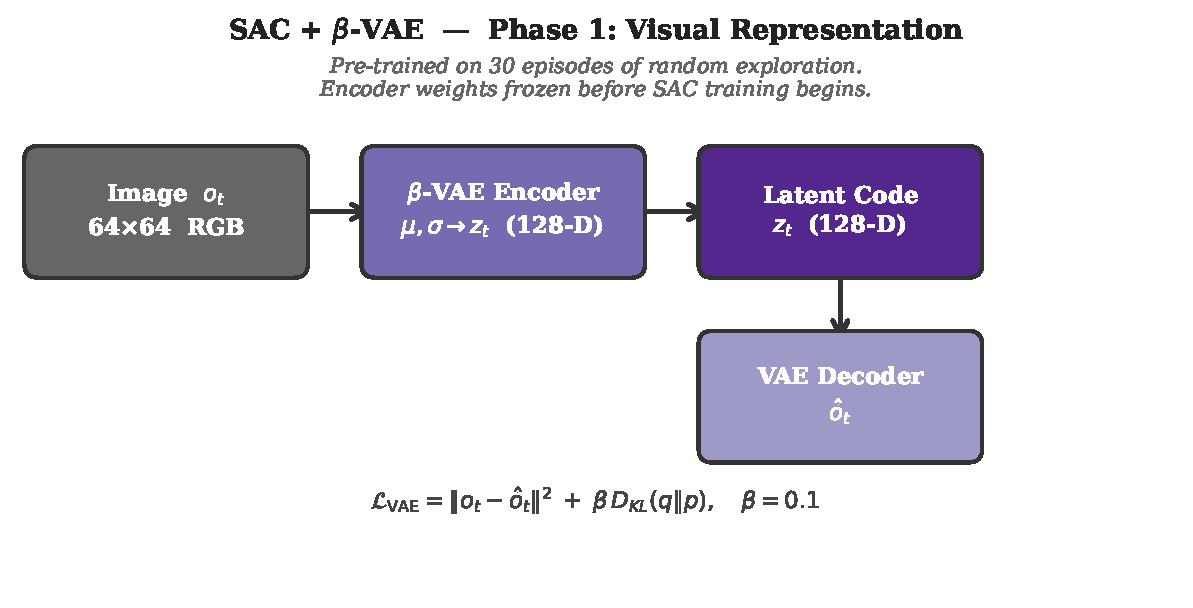
\includegraphics[width=0.68\textwidth]{figures/sac_vae.pdf}\\[0.6em]
  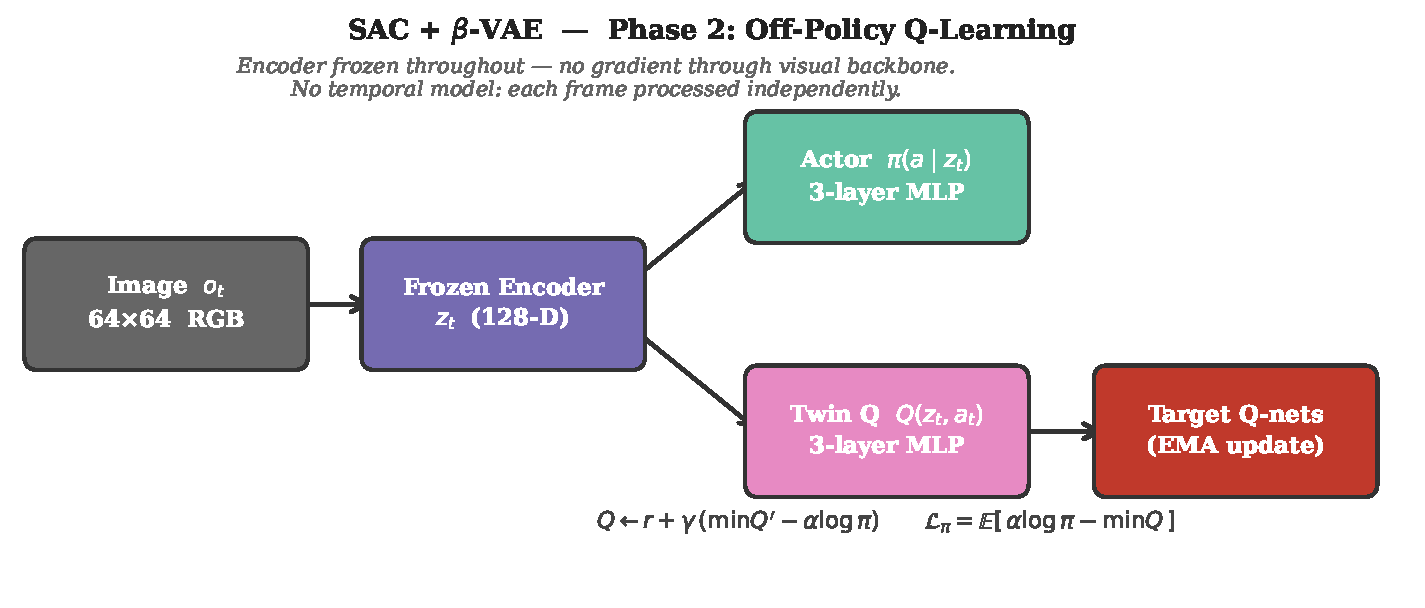
\includegraphics[width=0.85\textwidth]{figures/sac_rl.pdf}
  \caption{SAC+VAE architecture.
    \emph{Top — Phase 1 (Visual Representation):} A $\beta$-VAE ($\beta{=}0.1$)
    is pre-trained on 30 random-exploration episodes.
    The encoder maps images to 128-D Gaussian latents; the decoder reconstructs
    observations for the combined loss.
    \emph{Bottom — Phase 2 (Q-Learning):} The encoder is frozen; SAC trains
    twin Q-networks and an EMA target on $(z_t,a_t,r_t,z_{t+1})$ replay tuples.
    No temporal model or recurrence — every frame is processed independently.}
  \label{fig:sac_arch}
\end{figure*}

\subsection{Training Protocol}

\paragraph{Dreamer.}
Five seed episodes are collected with a random policy.
The world model and actor-critic are then updated for 50 gradient steps
per episode (\texttt{collect\_interval}=50), using batch size 50 with
sequence length 50.

\paragraph{SAC+VAE.}
Ten episodes of data are collected offline for VAE pre-training.
After VAE training, five seed episodes fill the replay buffer before
SAC updates begin. Per-step SAC updates are applied after each environment
step once the buffer exceeds the batch size.

\paragraph{Timing accounting.}
Wall-clock time is recorded from process launch, including all setup:
data collection and VAE training for SAC+VAE, and seed-episode collection
for Dreamer. This ensures the wall-clock comparison is end-to-end honest.

% ─────────────────────────────────────────────────────────────────────────────
\section{Experiments}

\subsection{Setup}
Experiments run on the DonkeyCar generated track
(\texttt{donkey-generated-track-v0}), a closed-loop circuit in the Unity
simulator. The host machine is an Apple Silicon Mac running the DonkeyCar
Unity app locally. Both methods use seed 42, RGB observations, no data
augmentation, and the variable-throttle action space.
Dreamer runs for 30 episodes (excluding 5 seed episodes);
SAC+VAE runs for 150 episodes (excluding 5 seed episodes).

\subsection{Results}

\begin{figure*}[t]
  \centering
  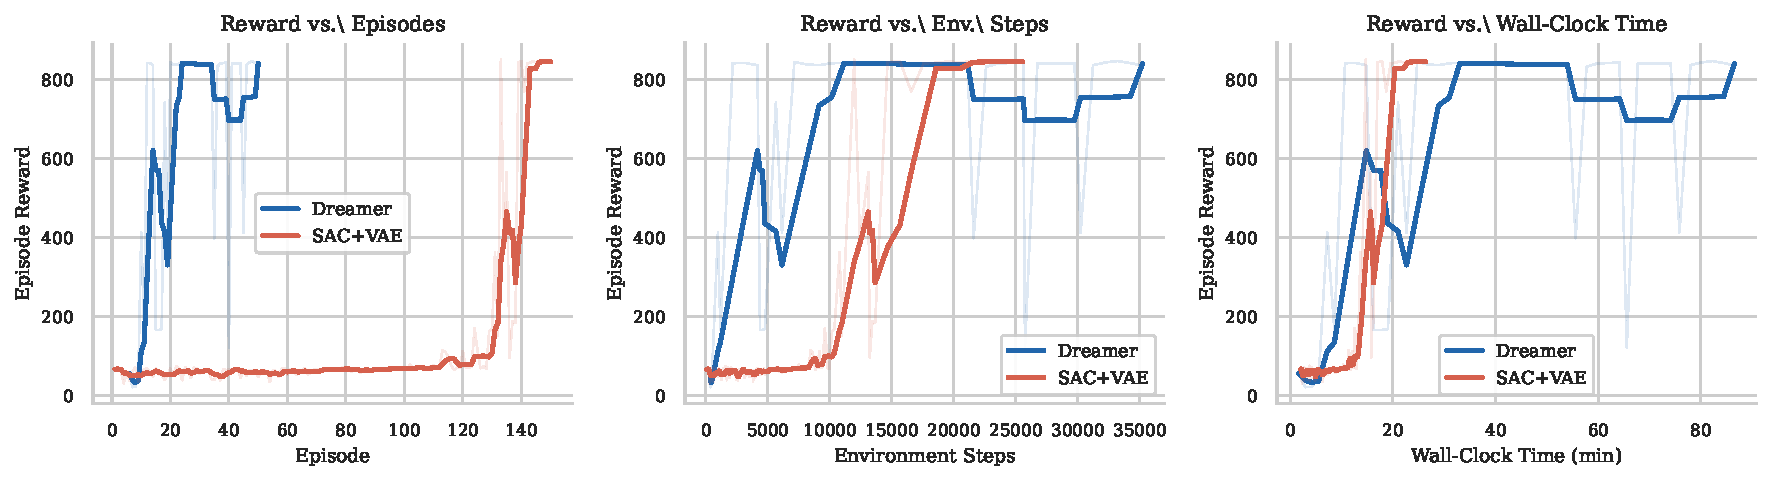
\includegraphics[width=\textwidth]{figures/training_curves.pdf}
  \caption{Training curves. \textcolor{dreamerblue}{\textbf{Dreamer}} (blue)
           vs.\ \textcolor{sacred}{\textbf{SAC+VAE}} (red).
           Shaded region shows raw episode values; solid line is a
           5-episode rolling mean.
           Left: reward vs.\ episodes. Centre: reward vs.\ environment steps.
           Right: reward vs.\ wall-clock time including all setup costs.}
  \label{fig:curves}
\end{figure*}

\begin{figure}[t]
  \centering
  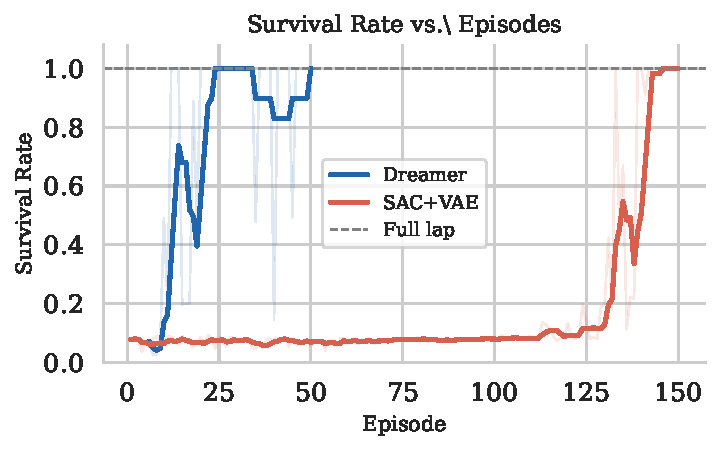
\includegraphics[width=\columnwidth]{figures/survival_rate.pdf}
  \caption{Survival rate (fraction of max episode length completed) vs.\
           episodes. A value of 1.0 indicates a full lap without crashing.}
  \label{fig:survival}
\end{figure}

Figure~\ref{fig:curves} shows learning curves and Figure~\ref{fig:survival}
shows survival rates.
Table~\ref{tab:results} summarises key metrics.

\begin{table}[h]
\centering\small
\caption{Summary of results on the generated track, single run.}
\label{tab:results}
\begin{tabular}{lcc}
\toprule
Metric & Dreamer & SAC+VAE \\
\midrule
Episodes to first full lap          & \textbf{16}  & 108   \\
Wall time to first full lap (min)   & 16.4         & \textbf{13.7} \\
Max episode reward                  & \textbf{845} & 860   \\
Mean reward (last 10 eps.)          & \textbf{840} & 790   \\
Actor loss trend                    & Stable       & Diverging \\
Total wall time (min)               & 43.5         & \textbf{41.6} \\
\bottomrule
\end{tabular}
\end{table}

\paragraph{Sample efficiency.}
Dreamer achieves its first complete lap at episode~16, requiring
7$\times$ fewer episodes than SAC+VAE (episode~108).
This reflects the core advantage of world-model learning: the agent
refines its policy using imagined experience rather than requiring
physical environment interaction for every gradient step.

\paragraph{Wall-clock time.}
When VAE pre-training and data collection are included in SAC+VAE's
wall-clock budget, the time to first full lap is comparable:
16.4 min for Dreamer vs.\ 13.7 min for SAC+VAE.
The world model therefore pays for itself in real time,
despite requiring more complex training infrastructure.

\paragraph{Policy stability.}
Dreamer's actor loss converges to approximately $-1.8$ and remains
stable throughout training (Figure~\ref{fig:curves}).
SAC+VAE exhibits monotonically diverging actor loss
(reaching $-34$ by episode~150), a symptom of Q-value overestimation
common when a frozen encoder prevents the representation from adapting
to correct bootstrapping errors~\cite{laskin2020curl}.
The divergence does not prevent the agent from learning a functional
policy in this environment, but it raises concerns about stability
in more complex tasks or over longer training horizons.

% ─────────────────────────────────────────────────────────────────────────────
\section{Discussion}

\subsection{Reward Transferability}
The survival + throttle reward is the primary design choice enabling
sim-to-real transfer. Pilot experiments using CTE-based rewards produced
policies that performed well in simulation but failed on hardware because
the on-board controller had no mechanism to compute CTE.
The throttle component naturally encourages speed management:
the agent learns to slow in tight corners to survive longer,
producing smoother trajectories than a fixed-throttle baseline.

\subsection{Limitations}
Results are from a single random seed on a single track;
statistical significance requires multiple seeds.
The SAC+VAE Q-overestimation issue may be addressed by
layer-normalised critics~\cite{bjorck2021high} or by end-to-end
encoder training, at the cost of additional complexity.
Real-car experiments are ongoing and not yet included in this report.

\subsection{Future Work}
\begin{itemize}[leftmargin=1.2em, itemsep=1pt, topsep=2pt]
  \item Multiple seeds (3--5) for statistically valid comparisons.
  \item Warehouse track (\texttt{donkey-warehouse-v0}) to test generalisation.
  \item Real Raspberry Pi~5 deployment results with lap-time comparison.
  \item Ablation: hflip augmentation, model size, KL balance coefficient.
  \item Twohot distributional critic (DreamerV3) for improved value estimation.
\end{itemize}

% ─────────────────────────────────────────────────────────────────────────────
\section{Conclusion}

We have shown that Dreamer achieves 7$\times$ greater sample efficiency
than SAC+VAE on the DonkeyCar generated track, while maintaining stable
policy gradients and comparable wall-clock training time.
The principled reward design—survival bonus plus throttle, without
cross-track error—enables direct transfer to the physical car without
simulator-specific signals, a prerequisite for real-world deployment.
These results motivate further investigation of model-based RL as a
practical approach to autonomous miniature vehicle navigation.

% ─────────────────────────────────────────────────────────────────────────────
\section*{Acknowledgements}
Experiments were conducted using the DonkeyCar simulator and the
\texttt{gym\_donkeycar} library. The Dreamer implementation is based on
the original PyTorch codebase adapted for embedded deployment.

% ─────────────────────────────────────────────────────────────────────────────
\bibliographystyle{abbrv}
\bibliography{refs}

\end{document}
